\begin{figure}
  \centering
  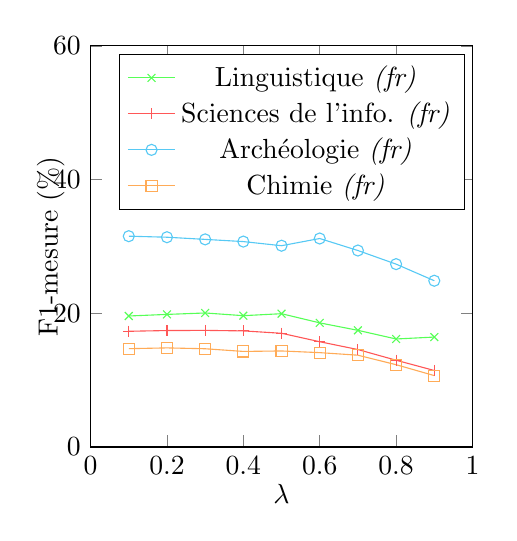
\begin{tikzpicture}
    \pgfkeys{/pgf/number format/.cd, fixed}
    \begin{axis}[x=0.4\linewidth,
                 xtick={0, 0.2, ..., 1.0},
                 xmin=0,
                 xmax=1.0,
                 xlabel=$\lambda$,
                 x label style={yshift=.34em},
                 y=0.007\linewidth,
                 ytick={0, 20, ..., 100},
                 ymin=0,
                 ymax=60,
                 ylabel=F1-mesure (\%),
                 y label style={yshift=-1.1em}]
      \addplot[green!66, mark=x] coordinates{
        (0.1, 19.5942)
        (0.2, 19.8314)
        (0.3, 20.0452)
        (0.4, 19.6420)
        (0.5, 19.9371)
        (0.6, 18.5649)
        (0.7, 17.4499)
        (0.8, 16.1558)
        (0.9, 16.4438)
      };
      \addplot[red!66, mark=+] coordinates{
        (0.1, 17.3100)
        (0.2, 17.4176)
        (0.3, 17.4420)
        (0.4, 17.3653)
        (0.5, 17.0094)
        (0.6, 15.7458)
        (0.7, 14.5758)
        (0.8, 12.9788)
        (0.9, 11.4421)
      };
      \addplot[cyan!66, mark=o] coordinates{
        (0.1, 31.5290)
        (0.2, 31.3748)
        (0.3, 31.0511)
        (0.4, 30.7214)
        (0.5, 30.1052)
        (0.6, 31.1819)
        (0.7, 29.3852)
        (0.8, 27.3498)
        (0.9, 24.8661)
      };
      \addplot[orange!66, mark=square] coordinates{
        (0.1, 14.7061)
        (0.2, 14.8227)
        (0.3, 14.6960)
        (0.4, 14.2947)
        (0.5, 14.3646)
        (0.6, 14.1136)
        (0.7, 13.7321)
        (0.8, 12.3091)
        (0.9, 10.6809)
      };
      \legend{Linguistique \textit{(fr)}, Sciences de l'info. \textit{(fr)}, Archéologie \textit{(fr)}, Chimie \textit{(fr)}};
    \end{axis}
  \end{tikzpicture}
  \caption{Performance de TopicCoRank, appliqué aux collections Termith, lorsque le paramètre $\lambda$ varie
           \label{fig:lambda_variations_termith}}
\end{figure}

